\documentclass[hyperref=colorlinks]{beamer}
\mode<presentation>
\usetheme{iclpt}
\setbeamertemplate{navigation symbols}{}
\setbeamertemplate{headline}{
\begin{beamercolorbox}[leftskip=.2cm,rightskip=.2cm,topskip=.2cm,ht=1.1cm,dp=0.1cm,wd=\textwidth]{institute in head/foot}
  
\includegraphics[height=1cm]{icl.pdf}
  \hfill
  
\includegraphics[height=1cm]{../Pics/CMS-Color.pdf}
\end{beamercolorbox}
}
\setbeamertemplate{footline}{
\begin{beamercolorbox}[ht=.55cm,dp=0.4cm,wd=\textwidth,leftskip=.3cm]{author in head/foot}%
  \begin{minipage}[c]{5cm}%
    \usebeamerfont{author in head/foot}
    \insertshortauthor 
    \insertshorttitle
    \end{minipage}\hfill%
  \insertframenumber{} / \pageref{lastframe}
  \hfill
  \begin{minipage}{6cm}
    \hfill
  \end{minipage}
\end{beamercolorbox}%
}

\usepackage{color}
\usepackage{tabularx,colortbl}
\usepackage{graphicx}
\usepackage{pdfpages}
\usepackage{feynmp}
\usepackage{multirow}
\DeclareGraphicsRule{*}{mps}{*}{}

\title{\vspace{-0.2cm} Trigger Efficiencies from 2015D}
%\subtitle{This result: HIG-15-012 \\ Contributing analyses: HIG-13-030, HIG-14-038, EXO-12-055}
\author[P. Dunne]{\underline{P. Dunne} on behalf of the H$\rightarrow$invisible analysis group}
\titlegraphic{
  \vspace{-0.7cm}
  %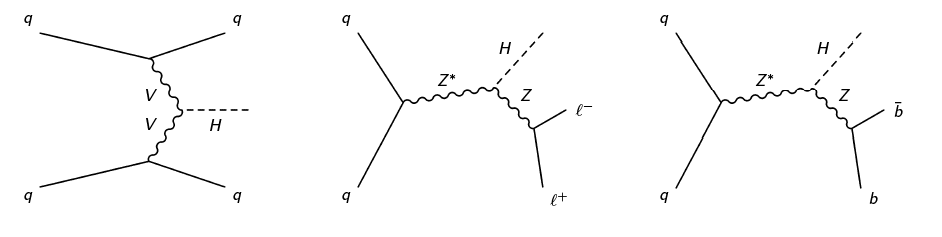
\includegraphics[width=\textwidth]{TalkPics/invcomb021213/feyndiags}
%% \begin{fmfgraph*}(100,70)
%%         \fmfleft{i1,i2}
%%         \fmfright{o1,o2,o3}
%%         \fmf{fermion}{i1,v1,o1}
%%         \fmf{fermion}{i2,v2,o3}
%%         \fmf{phantom,tension=4/5}{v1,v2}
%%         \fmffreeze
%%         \fmf{photon,label=$W,,Z$}{v1,v3}
%%         \fmf{photon,label=$W,,Z$}{v2,v3}
%%         \fmf{dashes}{v3,o2}
%%         \fmflabel{$q$}{i1}
%%         \fmflabel{$q$}{i2}
%%         \fmflabel{$q$}{o1}
%%         \fmflabel{$q$}{o3}
%%         \fmflabel{$H$}{o2}
%%       \end{fmfgraph*}
}
\date{}
\begin{document}
\begin{fmffile}{trigeff051015feyndiags}

%TITLE PAGE
\section{Title}
\begin{frame}
  \titlepage
  
\end{frame}

%!!CLOSURE TEST STATEMENT PU jet ID
%OUTLINE
\begin{frame}
  \frametitle{Introduction}
  \scriptsize
    \vspace{-.2cm}
    \begin{block}{\footnotesize Overview}
      \begin{itemize}
      \item 50ns data trigger efficiencies shown previously
      \item Golden JSONs from 2015D 25ns data have come out in the last couple of weeks
      \item $\sim$225.57 $pb^{-1}$ of 25ns data processed
      \item Updated trigger efficiencies will be shown today
      \end{itemize}
    \end{block}
\end{frame}

\begin{frame}
  \frametitle{Trigger Efficiencies - first iteration}
  \scriptsize
  \begin{block}{}
    \begin{itemize}
    \item Trigger: HLT\_DiPFJet40\_DEta3p5\_MJJ600\_PFMETNoMu140
    \item Measure efficiency as a function of each variable
    \item Started by cutting on all other variables at trigger threshold
    \item MET and jet 2 $p_{T}$ turn ons found to cause inefficiency in other variables
    \item[-] Cuts tightened to: Jet 1 and 2 $p_{T}>80$ GeV, METnoMu$>300$ GeV, $\Delta\eta_{jj}>3.5$, $M_{jj}>600$ GeV
    \end{itemize}
  \end{block}
\end{frame}

\begin{frame}
  \frametitle{Trigger efficiencies}
  \scriptsize
  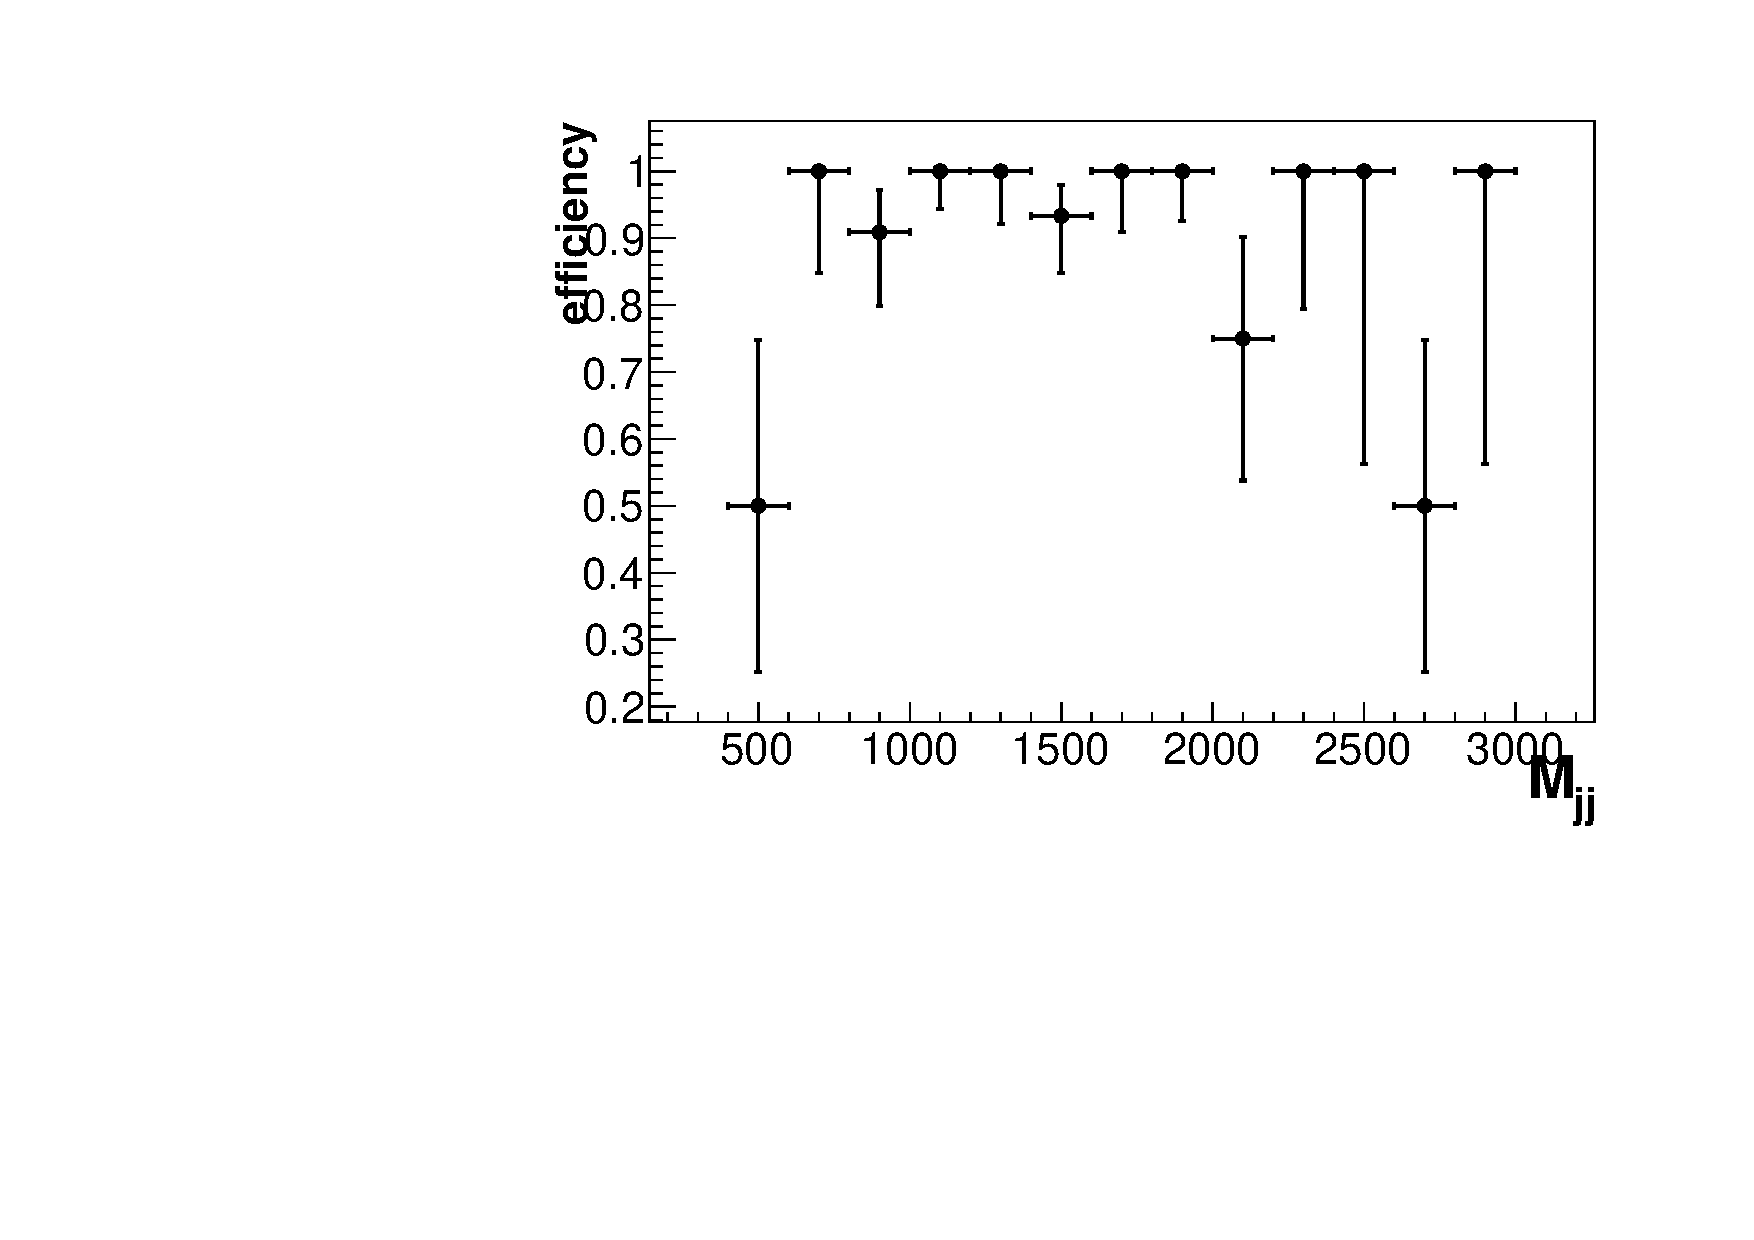
\includegraphics[width=.5\textwidth]{TalkPics/hinvtrigeff081015/output_2015Dtrigeff_071015/nunu_dijet_M.pdf}
  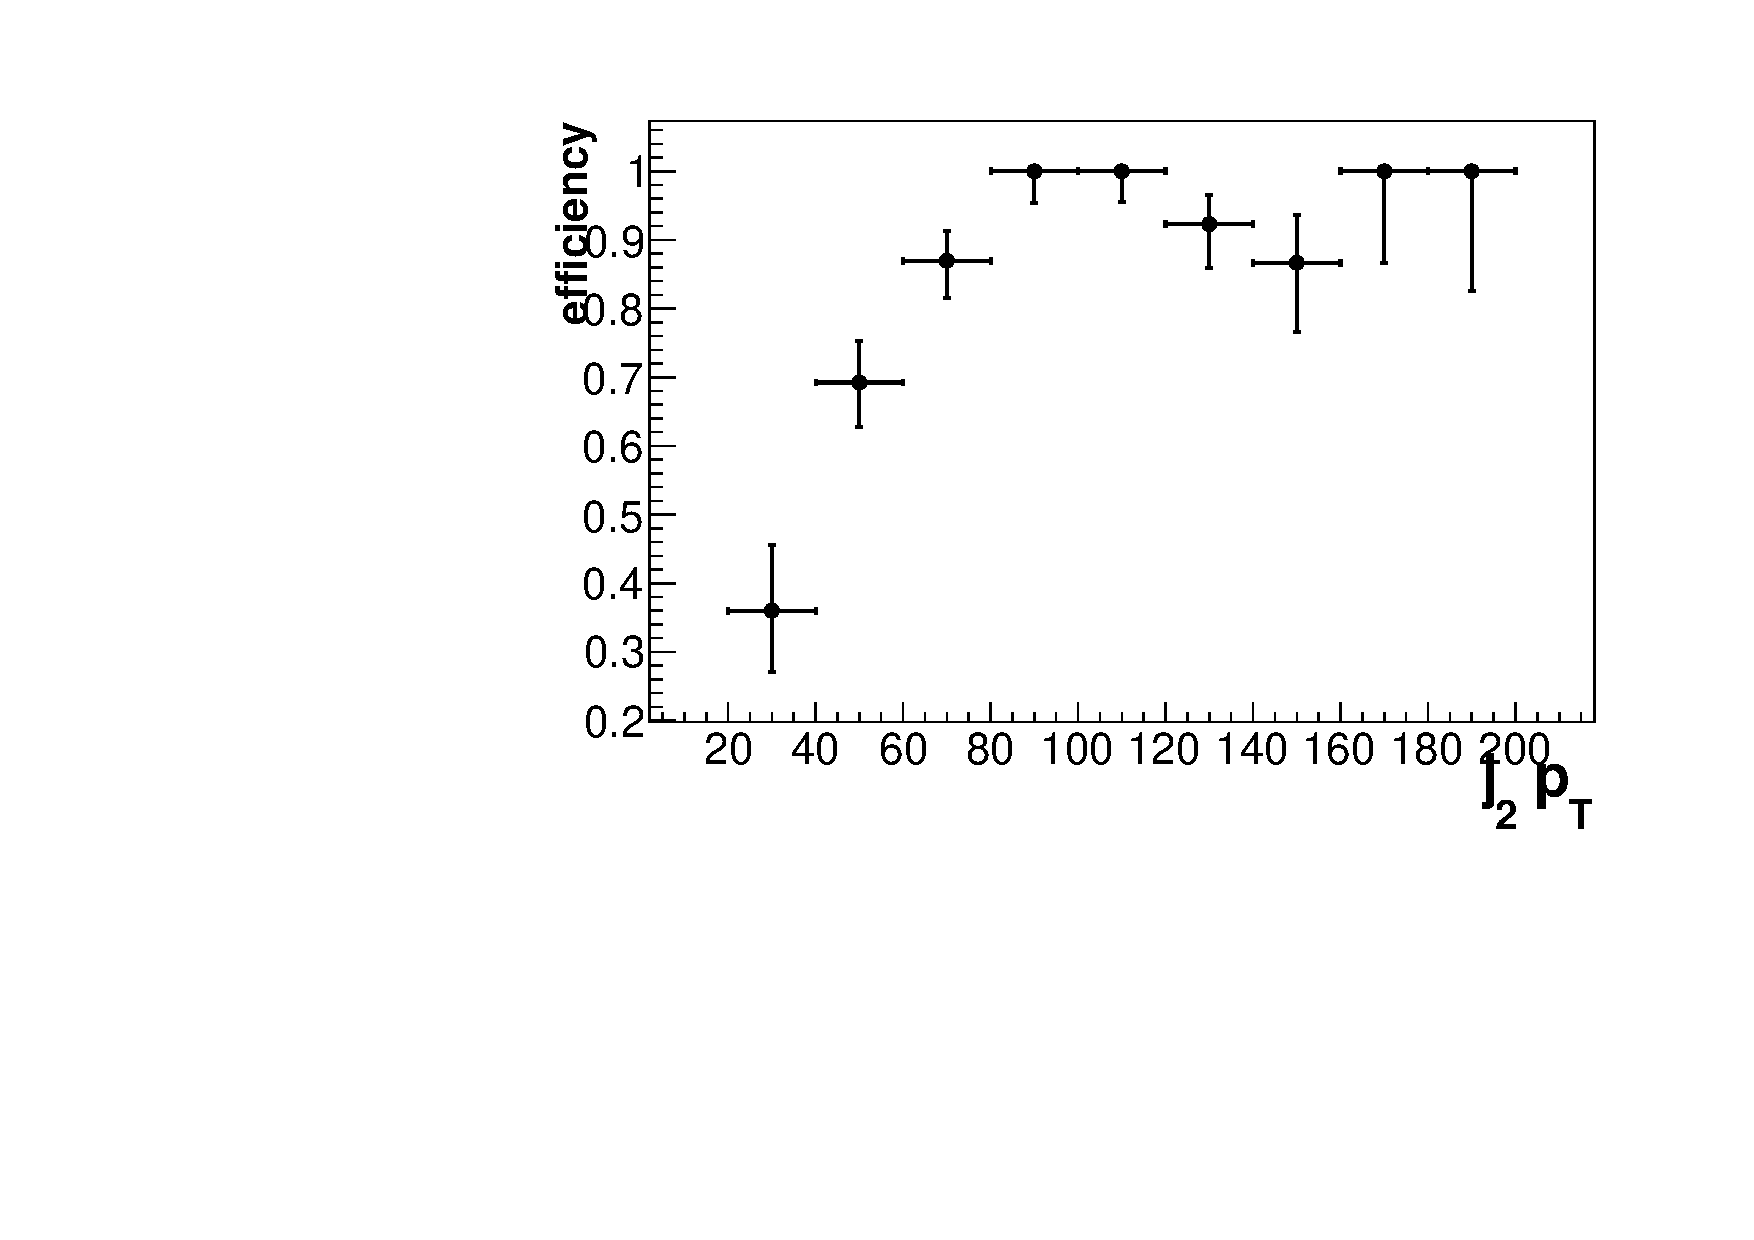
\includegraphics[width=.5\textwidth]{TalkPics/hinvtrigeff081015/output_2015Dtrigeff_071015/nunu_jet2_pt.pdf}
  \begin{block}{}
    \begin{itemize}
    \item Jet 2 $p_{T}$ turn on is quite slow, 95\% efficient only at 80 GeV
    \item[-] For the same trigger cut in run 1 the 95\% efficient point was $\sim$50 GeV
    \item[-] Jets are pfCHS from miniAOD with PF jet ID and old PU ID applied
    \end{itemize}
  \end{block}
\end{frame}

\begin{frame}
  \frametitle{Trigger efficiencies}
  \scriptsize
  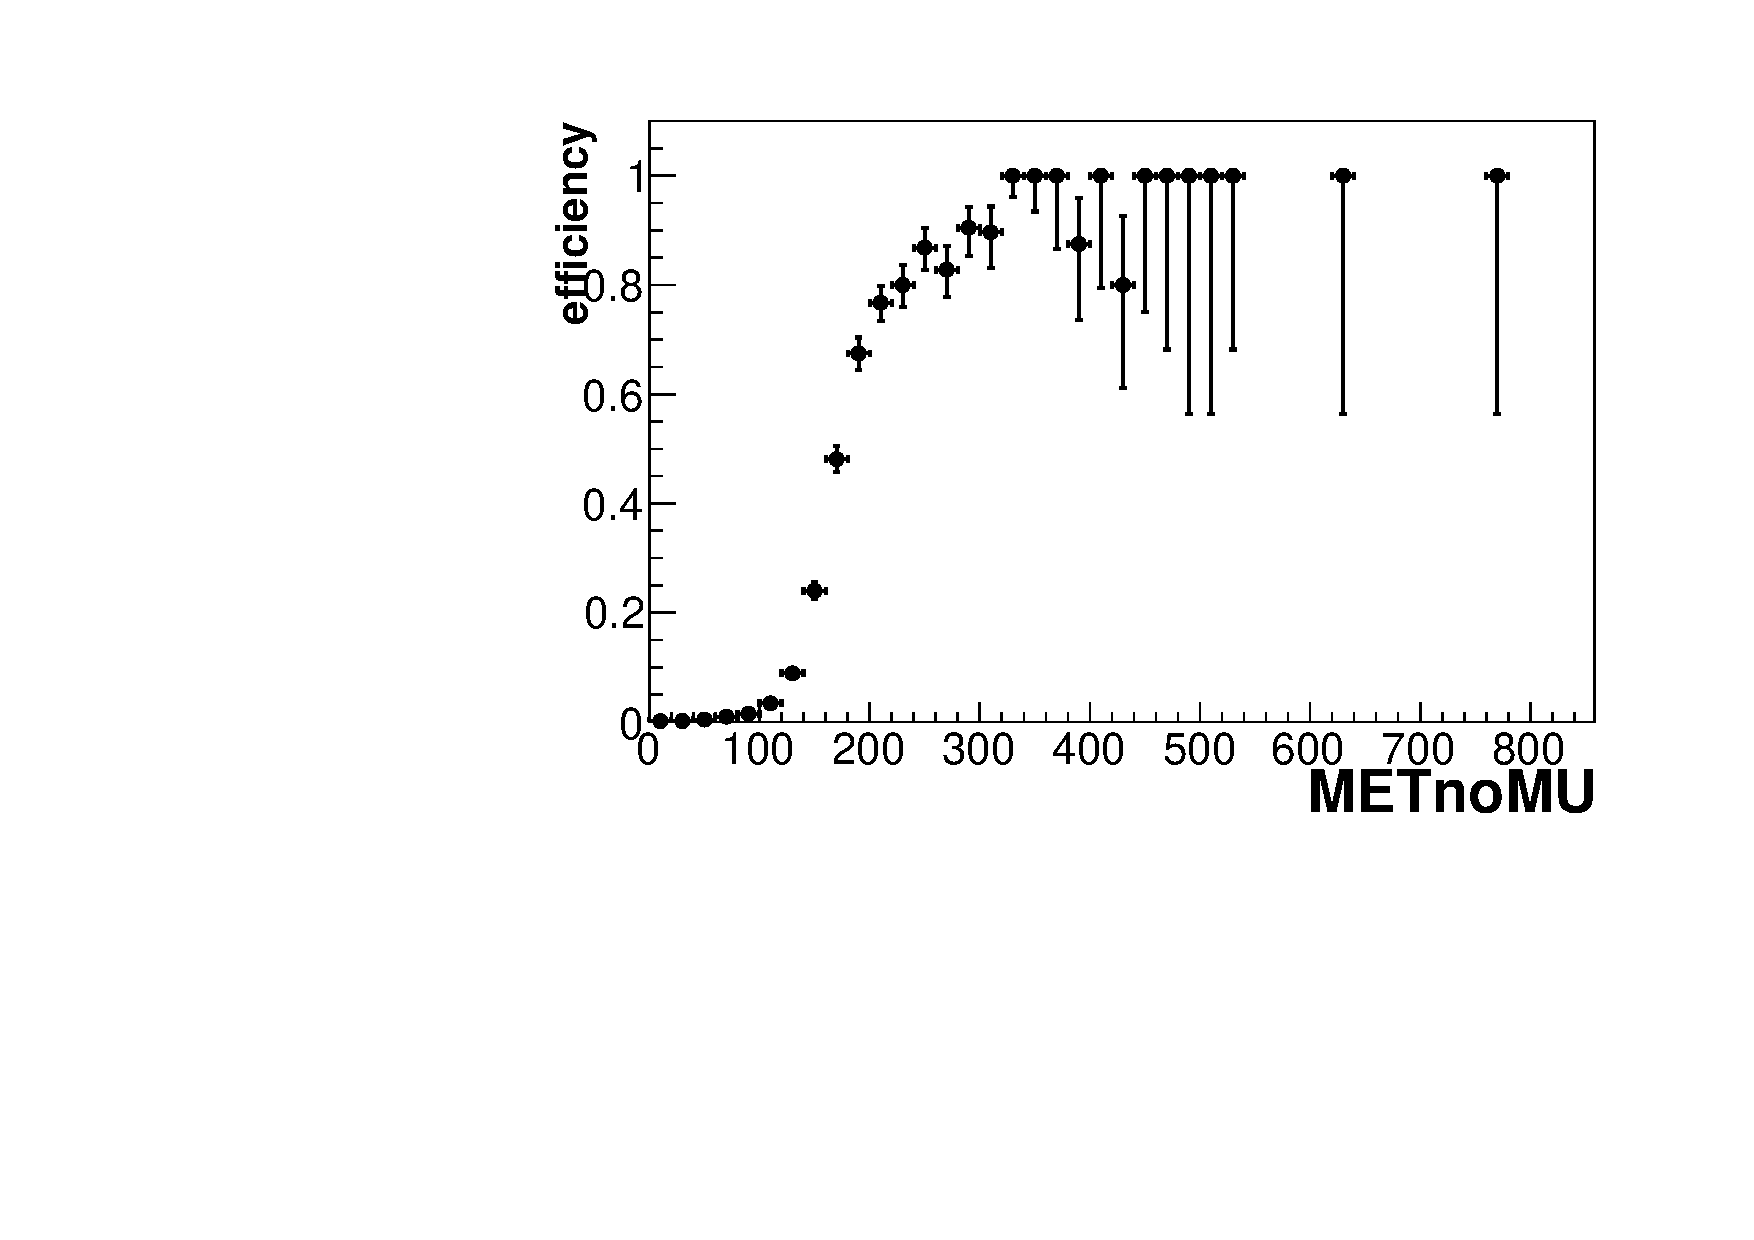
\includegraphics[width=.5\textwidth]{TalkPics/hinvtrigeff081015/output_2015Dtrigeff_071015/nunu_metnomuons.pdf}
  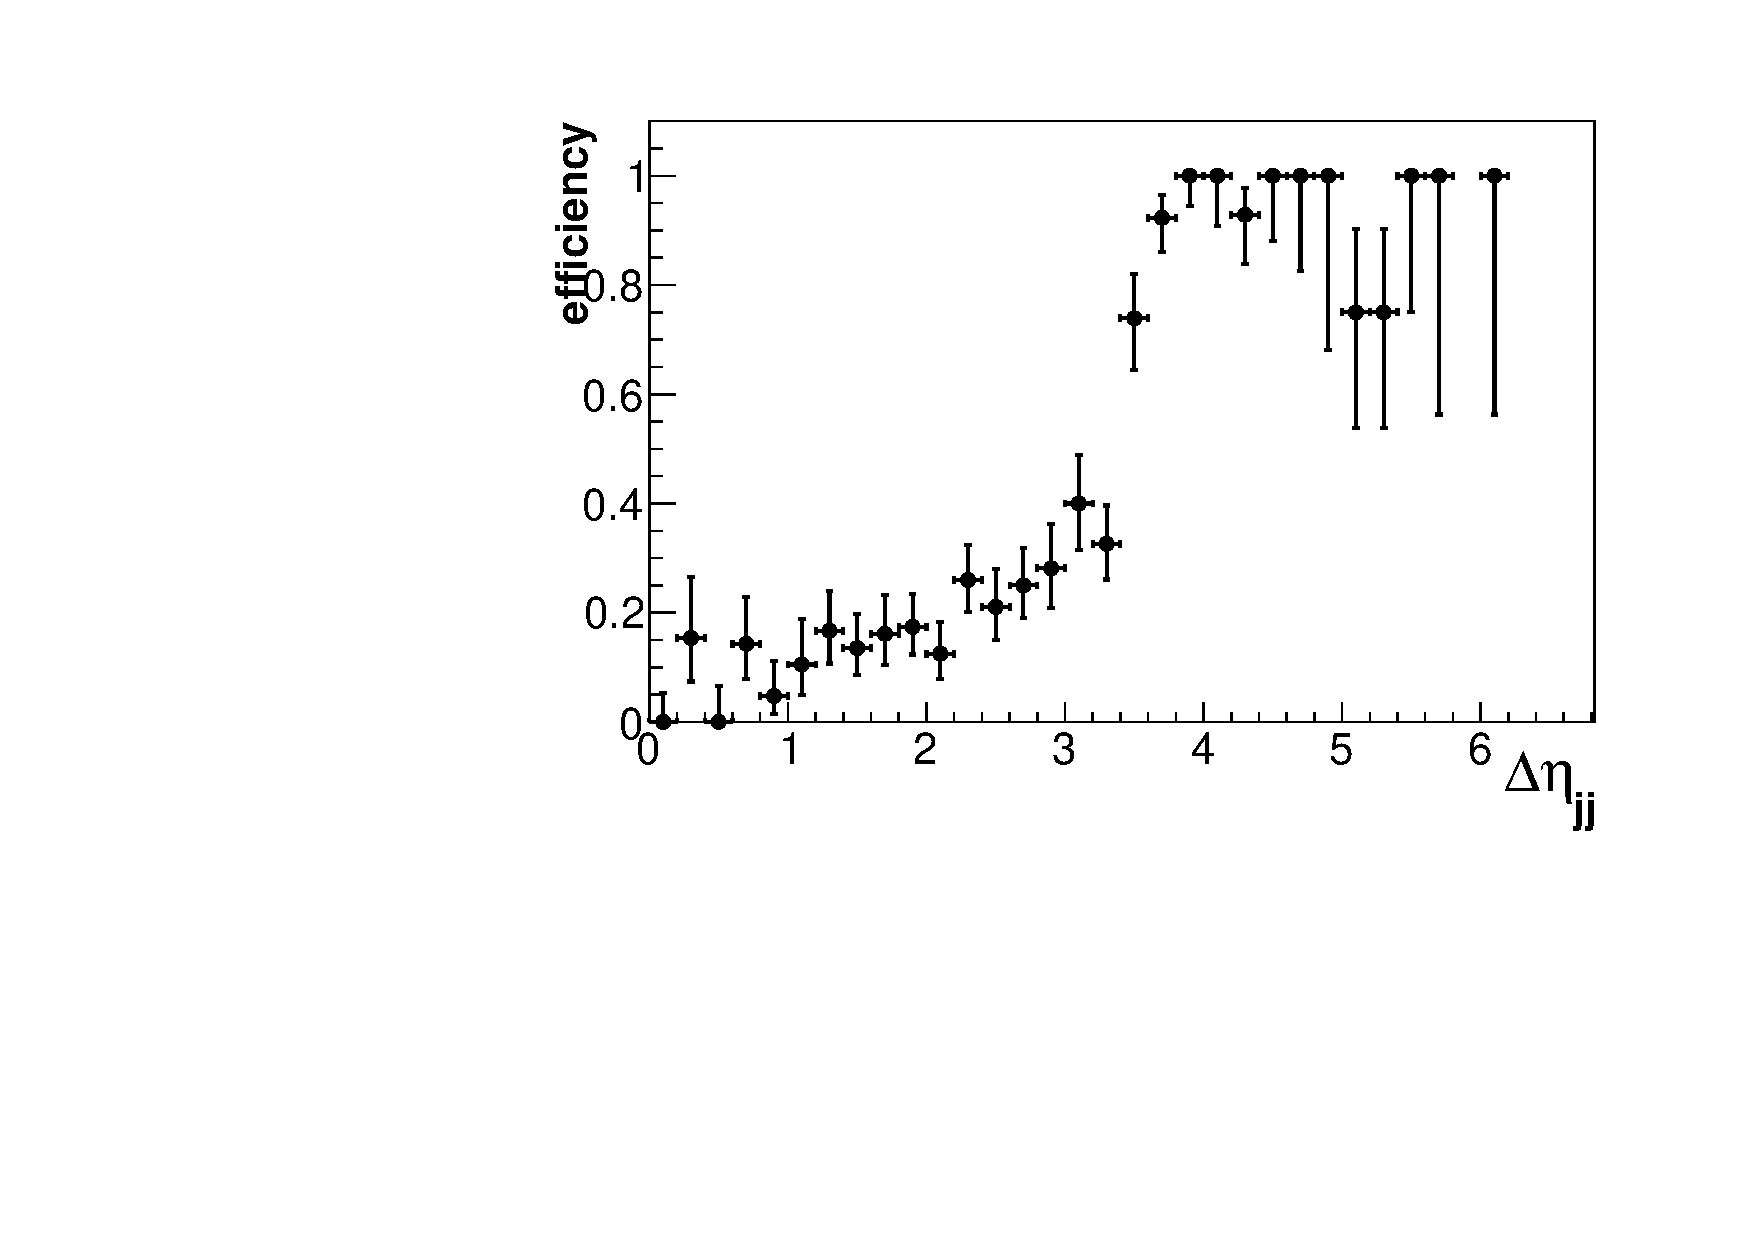
\includegraphics[width=.5\textwidth]{TalkPics/hinvtrigeff081015/output_2015Dtrigeff_071015/nunu_dijet_deta.pdf}
  \begin{block}{}
    \begin{itemize}
    \item METnoMu turn on has ``shelf'' at $\sim$200 GeV before becoming fully efficient at 300 GeV
    \item List of MET filters is that recommended by JetMET, HBHE filter recipe old as that on twiki leads to exception
    \end{itemize}
  \end{block}

\end{frame}

\begin{frame}
  \frametitle{Jet pt investigation}
  \scriptsize
  \begin{block}{}
    \begin{itemize}
    \item Measure efficiency separately for different jet configurations:
    \item[-] Both central, j2 forward j1 central, j1 forward j2 central, both forward
    \end{itemize}
  \end{block}
  \centering
  \begin{columns}
    \column{.5\textwidth}
  \begin{block}{Both central}
  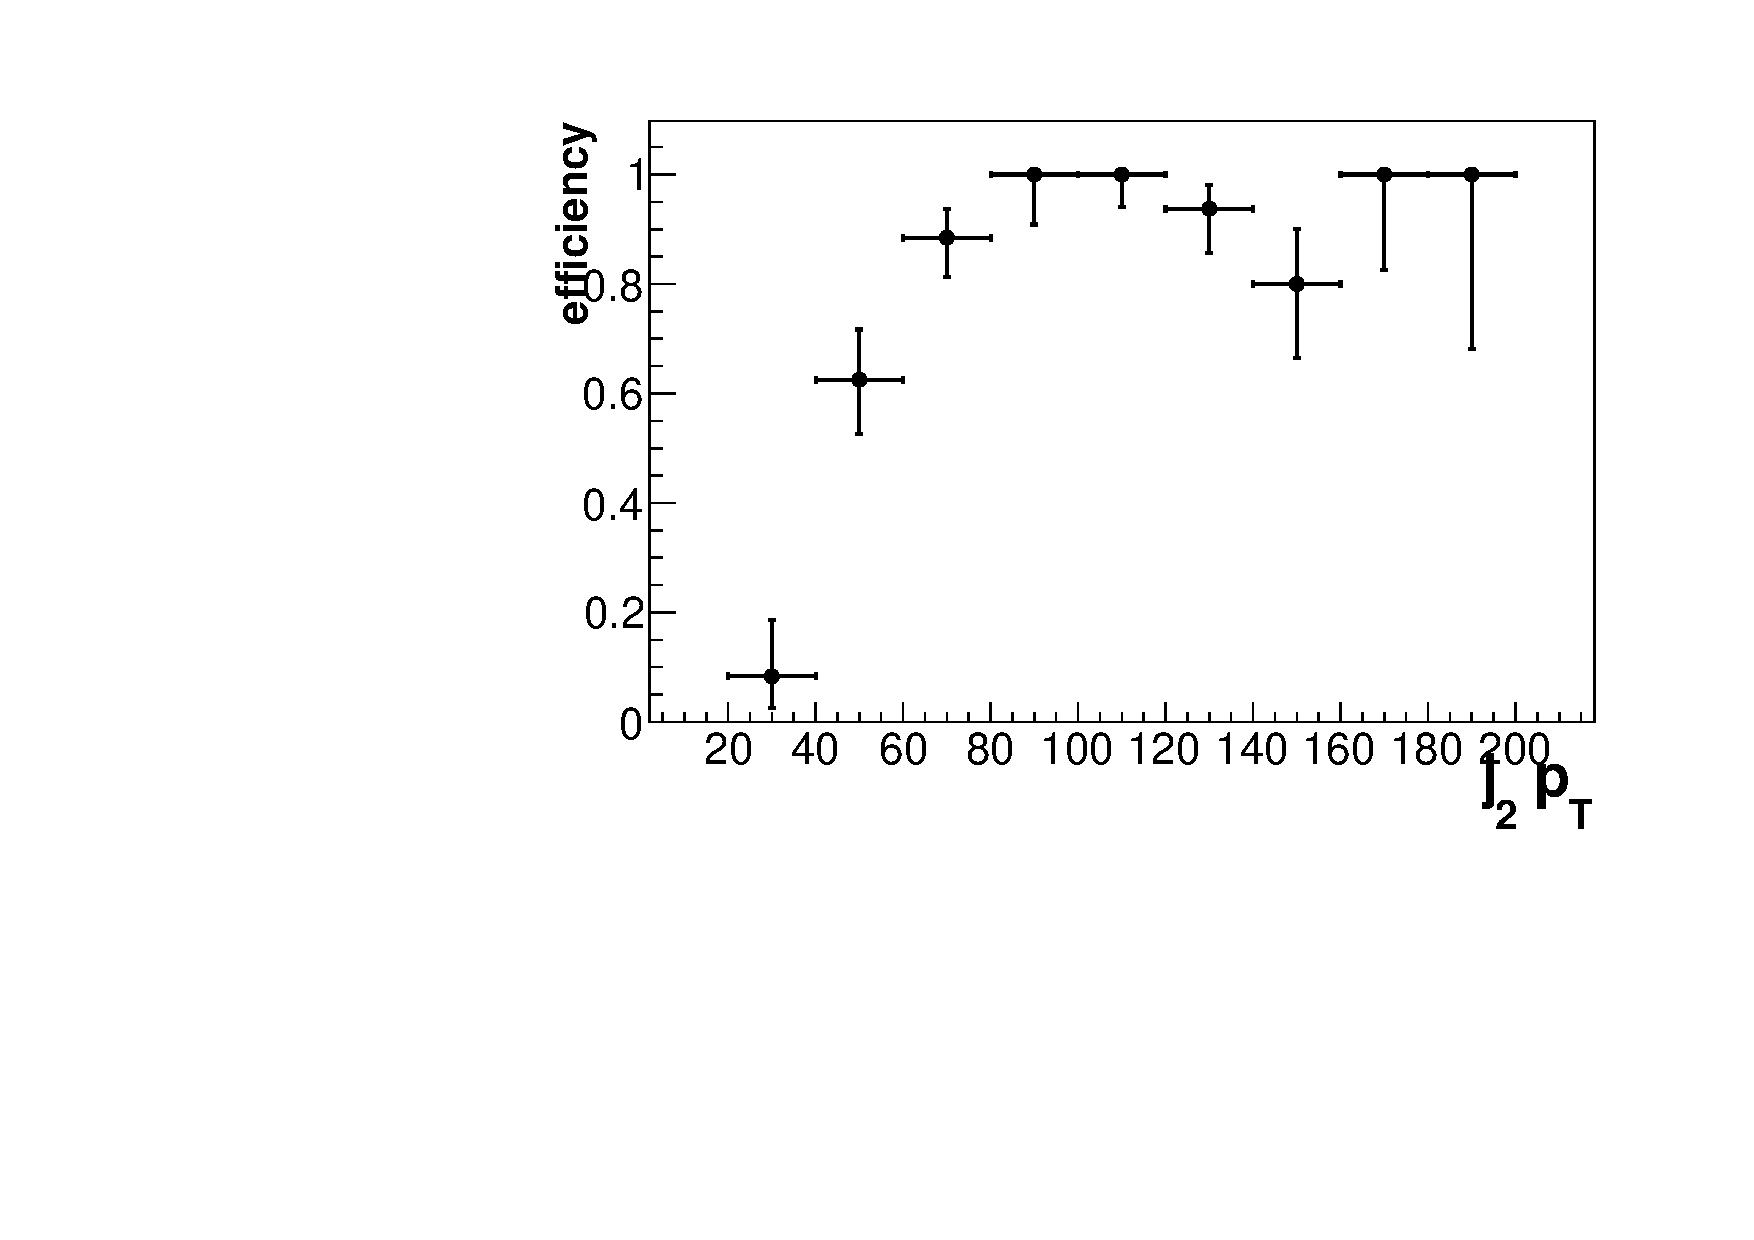
\includegraphics[width=\textwidth]{TalkPics/hinvtrigeff081015/output_2015Dtrigeff_bothcentral_071015/nunu_jet2_pt.pdf}
  \end{block}
  \end{columns}
\end{frame}

\begin{frame}
  \frametitle{Jet pt investigation}
  \scriptsize
  \begin{block}{}
    \begin{itemize}
    \item Measure efficiency separately for different jet configurations:
    \item[-] Both central, j2 forward j1 central, j1 forward j2 central, both forward
    \item Central defined as $|\eta|<3$
    \end{itemize}
  \end{block}
  \vspace{-.15cm}
  \begin{columns}
    \column{.5\textwidth}
  \begin{block}{j2 forward j1 central}
  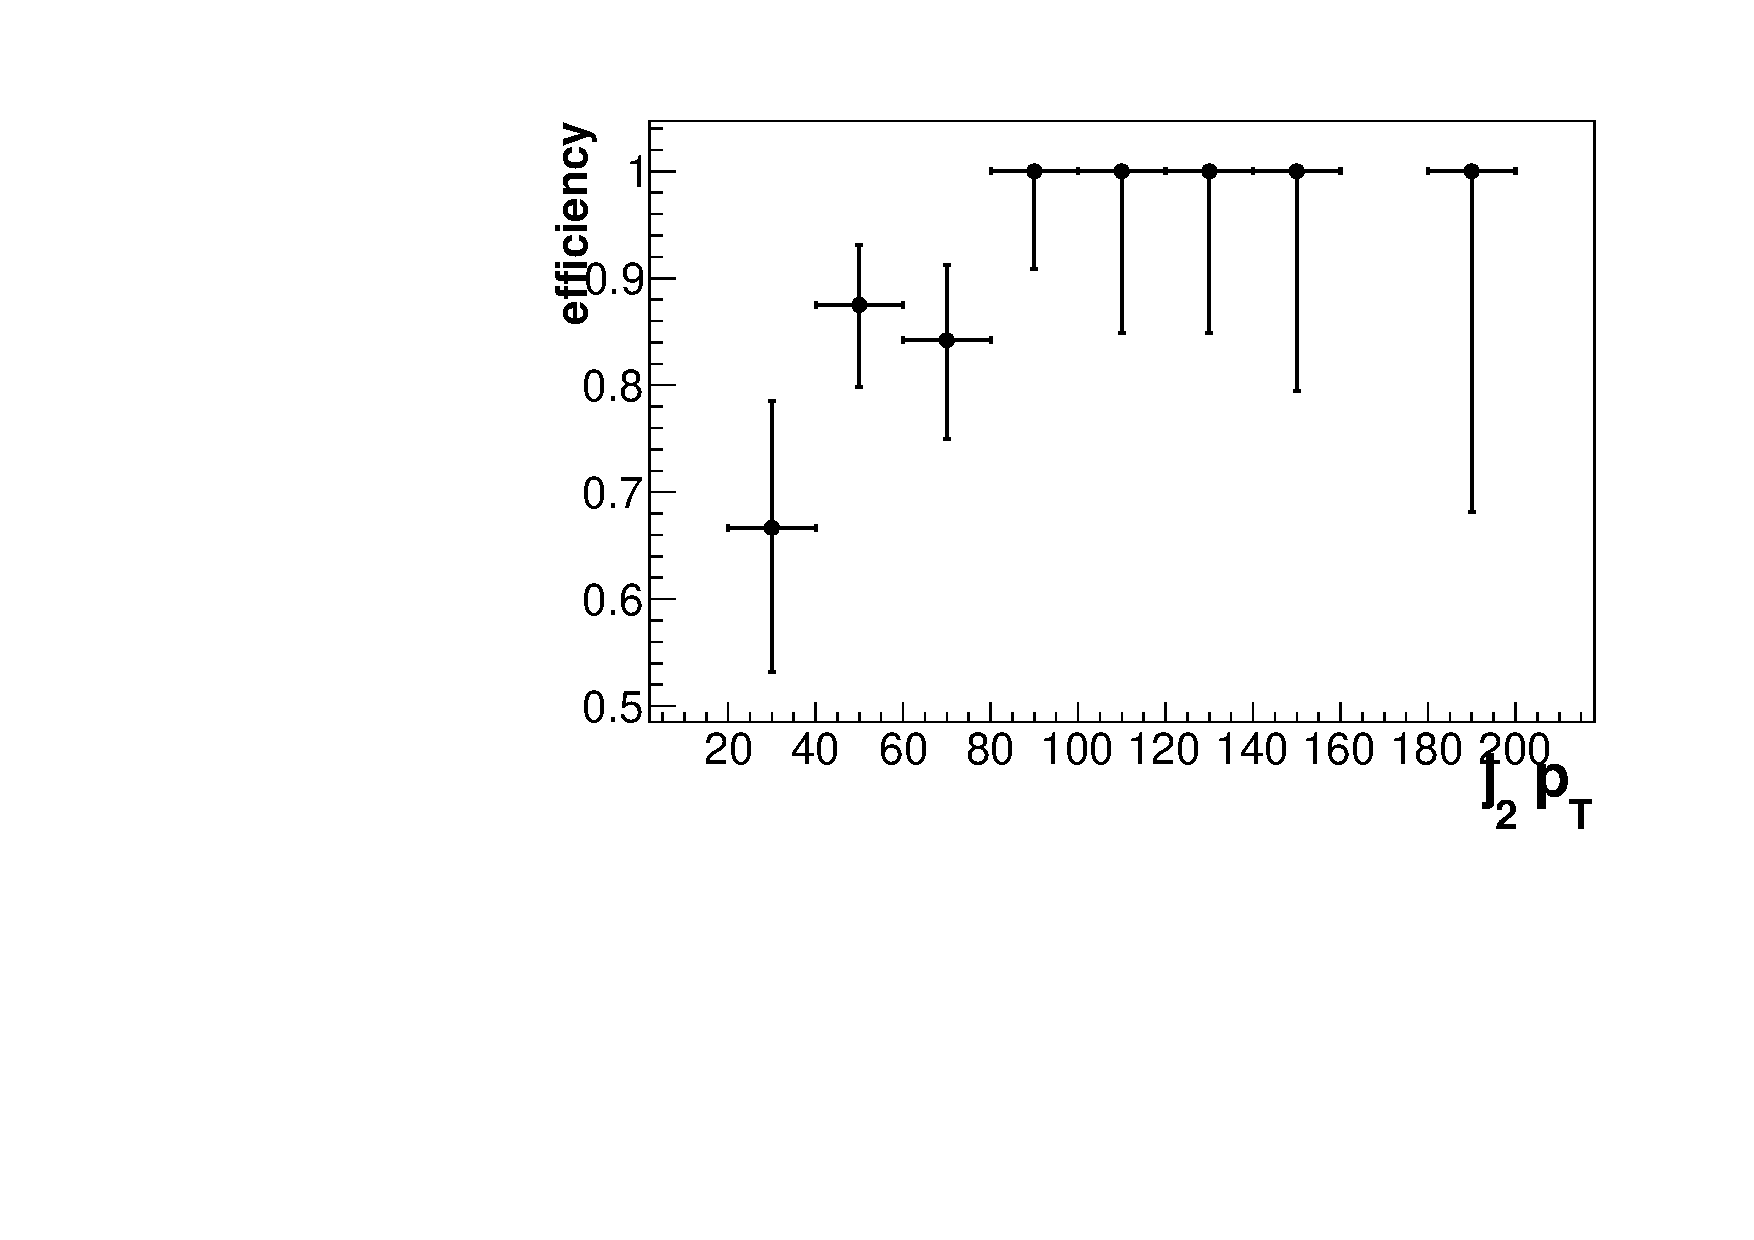
\includegraphics[width=\textwidth]{TalkPics/hinvtrigeff081015/output_2015Dtrigeff_j2forwardj1central_071015/nunu_jet2_pt.pdf}
  \end{block}
    \column{.5\textwidth}
  \begin{block}{j1 forward j2 central}
  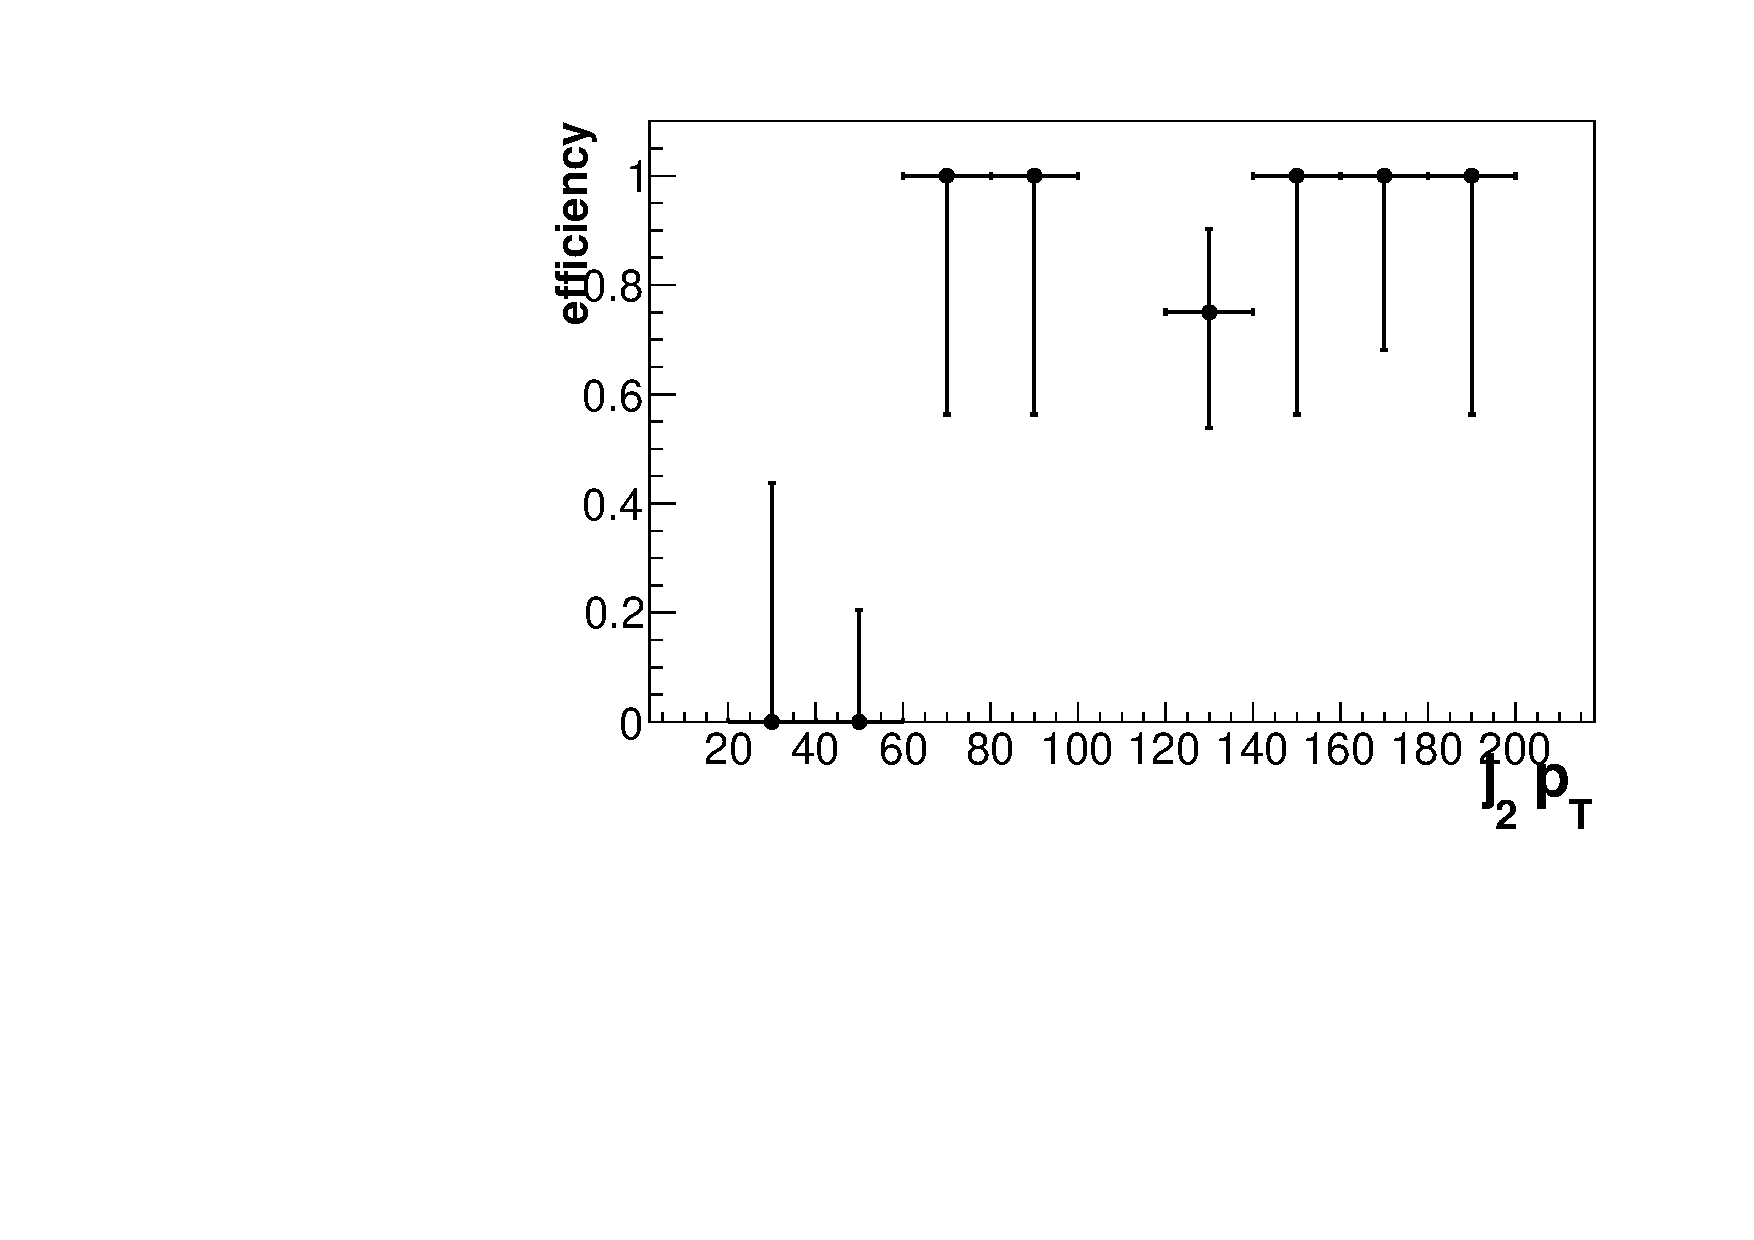
\includegraphics[width=\textwidth]{TalkPics/hinvtrigeff081015/output_2015Dtrigeff_j1forwardj2central_071015/nunu_jet2_pt.pdf}
  \end{block}
  \end{columns}  
\end{frame}

\begin{frame}
  \frametitle{Jet pt investigation}
  \scriptsize
  \begin{block}{}
    \begin{itemize}
    \item No events with both forward
    \item[-] Unsurprising as MET only considers central region
    \item Conclusions of $\eta$ dependence study limited by statistics
    \item[-] No obvious pattern
    \end{itemize}
  \end{block}
\end{frame}



\begin{frame}
  \frametitle{Summary}
  \label{lastframe}
  \begin{block}{}
    \scriptsize
    \begin{itemize}
    \item Trigger efficiencies from 25ns data shown:
    \item[-] MET shelf and slow jet 2 $p_{T}$ turn on interesting
    \item[-] $\Delta\eta_{jj}$ and $M_{jj}$ turn ons good
    \item We will continue to process data as it comes in to improve turn on curves
    \end{itemize}
  \end{block}
  \centering
\end{frame}

%UPDATED BACKUP
\begin{frame}
  \frametitle{Backup}
\end{frame}

\end{fmffile}
\end{document}
